\documentclass[../main.tex]{subfiles}
\chapter{Herleitung}
\label{c:herleitung}

\section[Homogene Transformationsmatrix]{Die homogene Transformationsmatrix}
\label{c:homtransform}

\begin{figure}
	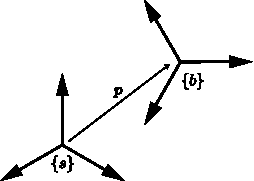
\includegraphics{frames}
	\caption{Transformation von space-frame $\{s\}$ nach body-frame $\{b\}$}
	\label{fig:frames}
\end{figure}

In Abbildung \ref{fig:frames} ist die Anordnung eines körperfesten Koordinatensystems $\{b\}$ (body-frame) in einem raumfesten Koordinatensystem $\{s\}$ (space-frame) dargestellt.
Ein Koordinatensystem wird als körperfest bezeichnet, wenn es sich relativ zum zugeordneten Körper nicht bewegt, bzw. der Körper sich nicht relativ zu diesem Bezugssystem ändert.
Das raumfeste Koordinatensystem wird als Ursprung des Raums angenommen; es bewegt sich nicht relativ zum Raum.
Die Anordnung von $\{b\}$ in $\{s\}$ kann durch die Position $\mathbf{p}$ und der Ausrichtung von $\{b\}$ in $\{s\}$-Koordinaten beschrieben werden.
Diese Orientierung wird durch eine Rotationsmatrix $\mathbf{R}$ beschrieben.
Die homogene Transformationsmatrix $\mathbf{T}$ ist die kombinierte Repräsentation von Orientierung und Position als Matrix \cite[Ch. 3.3.1]{KevinMLynch2017}:

\begin{equation}
	\label{eq:homTM}
	T = \begin{bmatrix}R & \vec{p}\\0 & 1\end{bmatrix} = \begin{bmatrix}r_{11} & r_{12} & r_{13} & p_1\\r_{21} & r_{22} & r_{23} & p_2\\r_{31} & r_{32} & r_{33} & p_3\\0 & 0 & 0 & 1\end{bmatrix}
\end{equation}

Häufig treten Transformationen als reine Translation oder Rotation auf.
Es bietet sich an für diese Fälle eine verkürzte Schreibweise einzuführen.
Eine reine Transformation wird beschrieben durch:

\begin{equation}
	\label{eq:translation}
	\transtm{t_x}{t_y}{t_z} = \begin{bmatrix}1 & 0 & 0 & t_x\\0 & 1 & 0 & t_y\\0 & 0 & 1 & t_z\\0 & 0 & 0 & 1\end{bmatrix}
\end{equation}

Bei einer reinen Transformation ist die Translationskomponente  $\mathbf{p} = \mathbf{0}$.
Die Rotationskomponente der homogenen Transformationsmatrix in Gleichung \ref{eq:homTM} wird beschrieben durch:
\begin{equation}
	\label{eq:rotationsmatrix}
	\begin{split}
		\rottm{\gamma}{\beta}{\alpha} & = R_{z}(\alpha ) \cdot R_{y}(\beta ) \cdot R_{x}(\gamma ) \\
			& = \begin{bmatrix}\c{\alpha} & -\s{\alpha} & 0\\\s{\alpha} & \c{\alpha} & 0\\0& 0& 1\end{bmatrix} \cdot
				\begin{bmatrix}\c{\beta} & 0& \s{\beta} \\0& 1& 0\\-\s{\beta} & 0& \c{\beta} \end{bmatrix} \cdot
				\begin{bmatrix}1& 0& 0\\0& \c{\gamma} & -\s{\gamma} \\0& \s{\gamma} & \c{\gamma} \end{bmatrix} \\
			& = \begin{bmatrix}
				\c{\alpha} \cdot \c{\beta} & \c{\alpha} \cdot \s{\beta} \cdot \s{\gamma} - \s{\alpha} \cdot \c{\gamma} & \c{\alpha} \cdot \s{\beta} \cdot \c{\gamma} + \s{\alpha} \cdot \s{\gamma} \\
				\s{\alpha} \cdot \c{\beta} & \s{\alpha} \cdot \s{\beta} \cdot \s{\gamma} + \c{\alpha} \cdot \c{\gamma} & \s{\alpha} \cdot \s{\beta} \cdot \c{\gamma} - \c{\alpha} \cdot \s{\gamma} \\
				-\s{\beta} & \c{\beta} \cdot \s{\gamma} & \c{\beta} \cdot \c{\gamma} \\
				\end{bmatrix} \\
		& \begin{aligned}
			\\
			\text{mit \quad}
				\s{x} & = \sin{(x)}\\
				\c{x} & = \cos{(x)}
		\end{aligned}
	\end{split}
\end{equation}

\section{Inverse von Transformationen}

Die Inverse einer Transformationsmatrix ist ebenfalls eine Transformationsmatrix der folgenden Form \cite[Prop. 3.15]{KevinMLynch2017}:
\begin{align*}
	T^{-1} & = \begin{bmatrix}R & \vec{p}\\0 & 1 \end{bmatrix}^{-1}\\
	& = \begin{bmatrix}R^\intercal & -R^\intercal \cdot \vec{p}\\0 & 1\end{bmatrix}
\end{align*}

\subsection[Translation]{Inverse der linearen Translation}

Bei einer linearen Translation ist die Rotationsmatrix die Einheitsmatrix.
Daher ergibt sich für die Translationskomponente:

\begin{equation}
	\label{eq:invtrans}
	\begin{split}
		-R^\intercal \cdot \vec{p} & = (-1) \cdot \begin{bmatrix}1 & 0 & 0\\0 & 1 & 0\\0 & 0 & 1\end{bmatrix}^\intercal \cdot \vec{p} \\
							 & = \begin{bmatrix}-1 & 0 & 0\\0 & -1 & 0\\0 & 0 & -1\end{bmatrix} \cdot \colvec{t_x}{t_y}{t_z} \\
							 & = \colvec{-t_x}{-t_y}{-t_z}
	\end{split}
\end{equation}

Somit ergibt sich für die Inverse der translatorischen Transformationsmatrix.

\begin{equation*}
	\tm{T^b_s}{t_x}{t_y}{t_z} ^{-1} = \tm{T^s_b}{-t_x}{-t_y}{-t_z}
\end{equation*}

\subsection[Rotation]{Inverse der Rotation um eine Achse}

Da bei der reinen Rotationsmatrix der Translationsvektor $p$ der Nullvektor ist, folgt, dass die Translationskomponente der inversen Transformationsmatrix ebenfalls der Nullvektor ist.
\begin{equation}
	\label{eq:inverserot}
	\begin{split}
		-R^\intercal \cdot \vec{p} & = (-1) \cdot \begin{bmatrix}1 & 0 & 0\\0 & 1 & 0\\0 & 0 & 1\end{bmatrix}^\intercal \cdot \colvec{0}{0}{0}\\
		& = \begin{bmatrix}-1 & 0 & 0\\0 & -1 & 0\\0 & 0 & -1\end{bmatrix} \cdot \colvec{0}{0}{0} \\
		& = \colvec{0}{0}{0}
	\end{split}
\end{equation}
Bei der Rotation um eine Achse ergibt sich die Rotationskomponente gemäß \ref{eq:rotationsmatrix} beispielhaft für Rotation um die z-Achse zu:
\begin{equation*}
	\begin{split}
		\rottm{0}{0}{\alpha} = & R_{z}(\alpha ) \cdot R_{y}(0) \cdot R_{x}(0) \\
							= & \begin{bmatrix}\cos \alpha & -\sin \alpha & 0\\\sin \alpha & \cos \alpha & 0\\0& 0& 1\end{bmatrix}
						\cdot	\begin{bmatrix}\cos 0 & 0& \sin 0 \\0& 1& 0\\-\sin 0 & 0& \cos 0 \end{bmatrix}
						\cdot	\begin{bmatrix}1& 0& 0\\0& \cos 0 & -\sin 0 \\0& \sin 0 & \cos 0 \end{bmatrix} \\
							= & \begin{bmatrix}\cos \alpha & -\sin \alpha & 0\\\sin \alpha & \cos \alpha & 0\\0& 0& 1\end{bmatrix}
	\end{split}
\end{equation*}

\begin{equation}
	\label{eq:sincossymm}
	\begin{split}
		\sin{-x} = & -\sin{x} \\
		\cos{-x} = & \cos{x}
	\end{split}
\end{equation}
Für die transponierte der Rotationskomponente ergibt sich mit den Symmetriebeziehungen gemäß Gleichung \ref{eq:sincossymm}:
\begin{equation*}
	\begin{split}
		R_{z}^\intercal(\alpha) = & \begin{bmatrix}\cos \alpha & -\sin \alpha & 0\\\sin \alpha & \cos \alpha & 0\\0& 0& 1\end{bmatrix}^\intercal \\
		= & \begin{bmatrix}\cos \alpha & \sin \alpha & 0\\-\sin \alpha & \cos \alpha & 0\\0& 0& 1\end{bmatrix} \\
		= & R_{z}(-\alpha)
	\end{split}
\end{equation*}
Damit folgt für die Inverse der Transformationsmatrix der reinen Rotation:
\begin{equation*}
	\tm{R^b_s}{0}{0}{\alpha} ^{-1} = \tm{R^s_b}{0}{0}{-\alpha}
\end{equation*}

\subsection{Notation der Indizes}

Um bei einer Transformation zu verdeutlichen aus welchem Koordinatensystem in welches andere Koordinatensystem transformiert wird, werden der Transformationsmatrix Indizes zugeordnet.

Das Subscript steht dabei für das Ausgangskoordinatensystem, das Superscript für das Zielkoordinatensystem.
Die zu Abb. \ref{fig:frames} gehörende Transformationsmatrix lautet daher:

\begin{equation*}
	T_s^b = \begin{bmatrix}R_s^b & \vec{p}\\0 & 1\end{bmatrix}
\end{equation*}
Bei einer Invertierung der Transformationsmatrix werden die Indizes getauscht, um zu beschreiben, dass die Transformationsrichtung nun vom body-frame $\{b\}$ in das space-frame $\{s\}$ erfolgt.

\section[Maschine]{Kinematik der Maschine}
Im Folgenden wird die Kinematik der Maschine in Abb. \ref{fig:maschine} erklärt und die mathematische Beschreibung ihrer Freiheitsgrade entwickelt.
Die Kinematik wird für diese Betrachtung, ausgehend von der Schnittstelle Maschinenbett-Werkstück, in zwei Pfade, den sogenannten kinematische Ketten, eingeteilt.

Das Maschinenbett wurde als Ursprung festgelegt, da sich sein Koordinatensystem auch bei realen Maschinen relativ zum Raum nicht bewegt, also raumfest ist.
Alle übrigen Teile der Maschine sowie das Werkstück sind mit einer mathematisch beschreibbaren Beziehung auf dieses Koordinatensystem referenziert.
Für beide kinematischen Ketten werden die Koordinatentransformation als Kombination von Transformationsmatrizen aufgestellt.
Um die Aufstellung nachvollziehbarer zu gestalten, beschreiben diese Transformationsmatrizen je einen primitiven Freiheitsgrad.
Beide Pfade werden vereint, um die gesamte Transformation als eine Matrix darstellen zu können.

Die erste kinematische Kette betrachtet, ausgehend von dem Ursprung, die Maschine mit den verfahrbaren Achsen bis zum Werkzeugkoordinatensystem.
Die zweite, in Richtung des Werkstücks, beschreibt die Position und Ausrichtung des Werkstückkoordinatensystems im Maschinenbett.
Um anschließend die Koordinatentransformation von dem Werkzeugkoordinatensystems in das Werkstückkoordinatensystems zu erhalten, werden die beiden Terme gleichgesetzt und nach Werkzeugkoordinaten aufgelöst.

\begin{figure}
	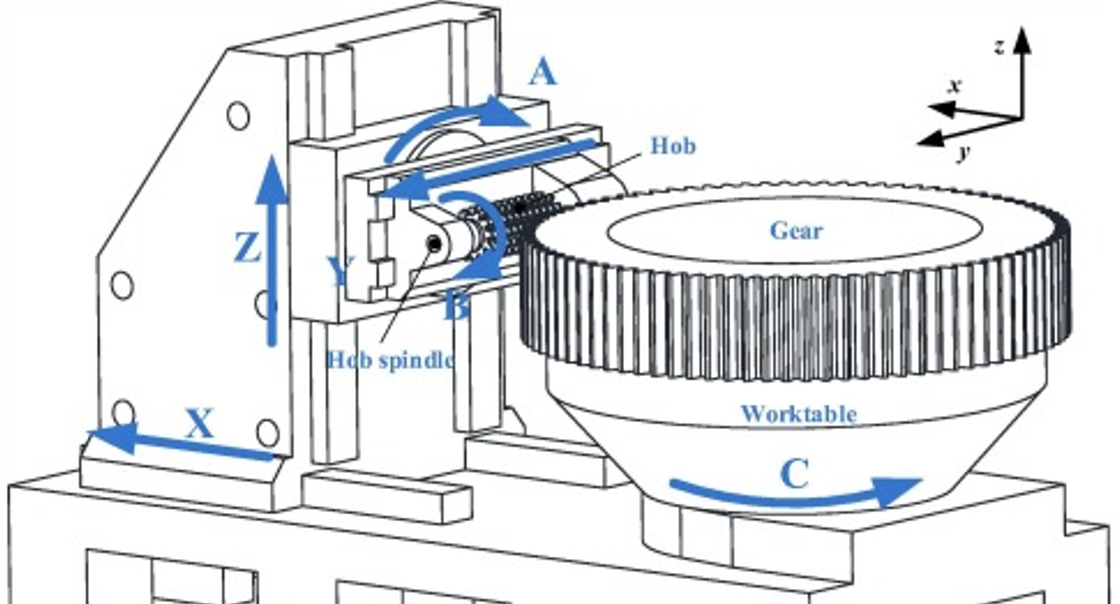
\includegraphics[width=12cm]{maschine_frei}
	\caption[Kinematik der Maschine]{Kinematik der Maschine mit Vorzeichenrichtung der Achsen}
	\label{fig:maschine}
\end{figure}

\subsection[Werkstück]{Kinematik der Werkstück-Seite}
\label{c:maschkinematik}
,,Die Kinematik des Verfahrens kann durch das Abwälzen einer Schnecke an einem Schneckenrad beschrieben werden.
Die Schnecke entspricht dem Werkzeug und das Schneckenrad dem Werkstück.'' \cite[4.2.3.2.1 Prozesskinematik]{FritzKlocke2016}.
Die Bewegung von Werkzeug und Werkstück ist somit über Vorschübe gekoppelt.

Für die kinematische Kette auf der Werkstückseite gehen in die Gleichungen \ref{eq:werkstuckv1} und \ref{eq:werkstuckv2} ein Offset des Werkstückkoordinatensystems zum Maschinenkoordinatensystem $\mathbf{p}_{\mathrm{offset}} = \tranvec{a}{b}{c}$ und der Verdrehwinkel $C$ ein.
Der Offset erlaubt es ein versetztes Aufspannen des Werkstücks darzustellen und ist im idealen Fall ein Nullvektor.
Dem Verdrehwinkel wird ein weiterer Offset $\gamma$ aufgeprägt.
Dieser erlaubt die Ausrichtung von Zahn und Zahnlücke des virtuellen Schneckengetriebes.
Bei vorverzahnten Bauteilen muss aufgrund des limitierten Bearbeitungsaufmaßes die Hülle der Soll-Geometrie in das zur Verfügung stehenden Material der Ist-Geometrie eingepasst werden.
Gleichzeitig gilt es bei Bearbeitung von wärmebehandelten Rohlingen die Einsatzhärtetiefe auf beide Zahnflanken der Zähne des fertigen Bauteils gleichmäßig zu erhalten.
Nach \cite{FritzKlocke2016} wird ,,[\dots] als Vorverzahnen [\dots] die Erzeugung der Zahnlückengeometrie im Rohling bezeichnet.''.
Es ist also notwendig die Zahnlücke des vorverzahnten Werkstücks mittig zu den Zähnen des Werkzeugprofils auszurichten.
Dieses Aufspannen ist in der Praxis fehlerbehaftet und in $\gamma$ kann dieser rotatorische Aufpannfehler bedacht werden.

$C$ ist außerdem eine Funktion des Werkzeugwinkels und des Achsvorschubes.
Nach \cite[Gl. (23.14)]{Matek2017} ist das Übersetzungsverhältnis eines Schneckengetriebes

\begin{equation}
	i = \frac{n_1}{n_2} = \frac{z_2}{z_1}
\end{equation}
\begin{eqdscr}{$n_1$, $n_2$}
	\item[$n_1$, $n_2$] Drehzahl der Schnecke, des Schneckenrades
	\item[$z_1$, $z_2$] Zähnezahl der Schnecke, des Schneckenrades
	\item[$i$] Übersetzungsverhältnis
\end{eqdscr}
Der Achsvorschub der $C$-Achse ist das Übersetzungsverhältnis des gedachten Schneckengetriebes.

\begin{equation*}
	\feed{C}{\wz} = \frac{n_{Schneidreihen}}{n_{Z"ahne}}
\end{equation*}
\begin{eqdscr}{$n_{Schneidreihen}$}
	\item[$\feed{C}{\wz}$] Vorschub der C-Achse bezogen auf das Werkzeug
	\item[$n_{Schneidreihen}$] Anzahl der Schneidreihen des Werkzeugs
	\item[$n_{Z"ahne}$] Zähnezahl des Werkstücks
\end{eqdscr}
Im Folgenden werden verfahrbaren Achsen der Maschine mit einem Großbuchstaben bezeichnet, die Achsen eines Koordinatensystems mit einem Kleinbuchstaben.
Der Hintergrund ist, dass hier beschriebene Maschine eine X-, Y- und Z-Achse haben, die zwar üblicherweise in Richtung der x-, y- und z-Achse des Maschinenbettkoordinatensystems zeigen, aber nicht zwingenderweise deckungsgleich sind.
Dabei liegt das Beispiel der Y-Achse der Maschine auf der Hand, die nur dann tatsächlich die selbe Richtung hat wie die y-Achse des Maschinenbettkoordinatensystems, wenn die  A-Achse nicht eingeschwenkt ist.
Die vollständige Formulierung des Werkstückwinkels $C$ lautet:

\begin{equation}
	\label{eq:wrkstwinkel}
	C = B \cdot{} \feed{C}{Wz} + \gamma
\end{equation}
\begin{eqdscr}{$\feed{C}{Wz}$}
	\item[$C$] Winkel des Werkstücks
	\item[$B$] Winkel des Werkzeugs
	\item[$\feed{C}{Wz}$] Achsvorschub der C-Achse
	\item[$\gamma$] Verdrehwinkel des Werkstücks zum Bearbeitungstisch
\end{eqdscr}
Zur Beschreibung der Kinematik können zwei verschiedene Varianten gewählt werden.
Sie unterscheiden sich durch die Reihenfolge der Freiheitsgrade Werkstückversatz und Maschinen-C-Achse in der kinematischen Kette.

\subsubsection[Versetzter Bearbeitungstisch]{Variante 1: Versetzter Bearbeitungstisch}

Bei Variante 1 liegt das Bauteil konzentrisch auf dem Bearbeitungstisch und das Paar dreht sich um die C-Achse.
Der Ursprung des Bearbeitungstisches mit C-Achse fällt nicht mit dem Maschinenbettkoordinatensystem zusammen, sondern ist um $\mathbf{p}_{\mathrm{offset}}$ versetzt.
Diese Variante ist in der Praxis verbreitet, um Maschinen zu kalibrieren und mögliche Betriebsschäden auszugleichen.
Die Transformation beschreibt die Position eines Werkstückpunktes im Koordinatensystem des Maschinenbetts.

\begin{equation}
	\label{eq:werkstuckv1}
	\vec{p}_\mathrm{m} = \transtm{a}{b}{c}
			\cdot{} \rottm{0}{0}{C}
			\cdot{} \vec{p}_\wst
\end{equation}

\subsubsection[Versetztes Werkstück]{Variante 2: Versetztes Werkstück}
Bei Variante 2 sind Bauteil und Bearbeitungstisch nicht konzentrisch.
Stattdessen sind Ursprung von Werkstück und Bearbeitungstisch um $\mathbf{p}_{\mathrm{offset}}$ versetzt.
Dieser dreht sich um die C-Achse, welche koaxial zur z-Achse des Maschinenbetts ist.
Diese Variante hat nur theoretische Bedeutung.

\begin{equation}
	\label{eq:werkstuckv2}
	\vec{p}_\mathrm{m} =
					\rottm{0}{0}{C}
			\cdot{} \transtm{a}{b}{c}
			\cdot{} \vec{p}_\wst
\end{equation}

\subsection[Werkzeug]{Kinematik der Werkzeug-Seite}
\label{c:werkzeugkinematik}
\begin{equation}
	\label{eq:werkzeug}
	\vec{p}_\mathrm{m} =  \transtm{X}{0}{Z}
	\cdot{} \rottm{A}{0}{0}
	\cdot{} \transtm{0}{Y}{0}
	\cdot{} \rottm{\pi/2}{0}{0}
	\cdot{} \rottm{0}{0}{B}
	\cdot{} \vec{p}_\wz
\end{equation}
Gleichung \ref{eq:werkzeug} beschreibt die Transformation eines Werkzeugpunktes in das Koordinatensystems des Maschinenbettes.
Diese kinematische Kette beinhaltet die verfahrbaren Achsen der Maschine mit ihrem jeweiligen Freiheitsgrad.

\begin{figure}
	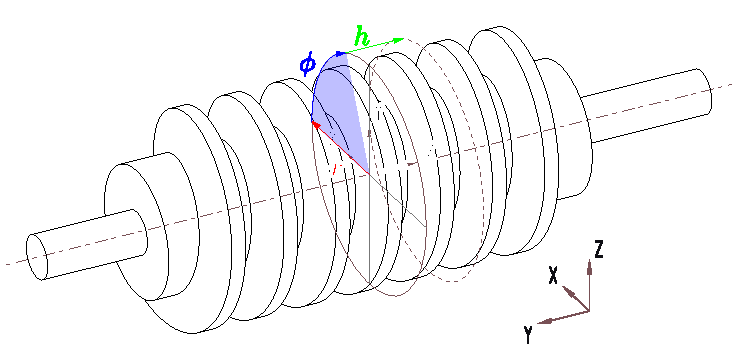
\includegraphics{hobspindle_coord}
	\caption{Ausrichtung des Werkzeugkoordinatensystems}
	\label{fig:hobspindle_coord}
\end{figure}
Es bietet sich an, das Koordinatensystem des Werkzeugs gemäß Abbildung \ref{fig:hobspindle_coord} zu definieren.
Wenn Drehachse und z-Achse des Werkzeugkoordinatensystems koaxial sind, kann die Beschreibung des Werkzeugs leicht in Zylinderkoordinaten erfolgen.
Dabei ist die Umrechnung von und nach kartesischen Koordinaten wenig Aufwand, vgl. Gleichung \ref{eq:wkzgkoord}.
\begin{equation}
	\label{eq:wkzgkoord}
	\vec{p}_{\mathrm{Wz,kart}}	= \begin{pmatrix}x \\ y \\ z \end{pmatrix}
	= \begin{pmatrix}r \cdot \cos{\phi} \\ r \cdot \sin{\phi} \\ h \end{pmatrix}
\end{equation}
Die Festlegung der positiven Richtung der z-Achse kann geschickt gewählt werden, sodass die Drehrichtung des Werkzeugs in seinem Koordinatensystem positiv definiert ist.
Der Spanabfall soll in Drehrichtung des Werkzeugs erfolgen, das heißt die Bewegung des Werkzeugs beim Schneiden des Werkstücks erfolgt also von ,,oben'' nach ,,unten''.
Daraus ergibt sich, dass die Ausrichtung der z-Achse in negativer Richtung der Maschinen y-Achse erfolgen muss.
Diese Ausrichtung des Werkstückkoordinatensystems erfordert das Einführen einer Transformationsmatrix zwischen der Werkzeugdrehmatrix und der Tangentialvorschub-Matrix.
Augenscheinlich handelt es sich dabei um eine viertel Umdrehung um die x-Achse des Maschinenkoordinatensystems.
\begin{equation*}
	\rottm{\pi/2}{0}{0}
	= \begin{bmatrix}1 & 0 & 0 & 0\\0 & 0 &-1 & 0\\0 & 1 & 0 & 0\\0 & 0 & 0 & 1\end{bmatrix}
\end{equation*}
Zur Vereinfachung der entstehenden Terme bietet sich das Zusammenfassen der Transformationsmatrizen zu einer Transformationsmatrix von Maschinenbett- in Werkzeugkoordinaten an:

\begin{equation*}
	T^\wz_\mathrm{m} = \transtm{X}{0}{Z}
				\cdot{} \rottm{A}{0}{0}
				\cdot{} \transtm{0}{Y}{0}
				\cdot{} \rottm{\pi/2}{0}{0}
				\cdot{} \rottm{0}{0}{B}
\end{equation*}

\subsection{Position der Maschinenachsen}
\label{c:maschkomppos}
Bei Gleichung \ref{eq:wrkstwinkel} wurde die Abhängig der C-Achsenposition von dem Winkel des Werkzeugs beschrieben.
Damit ist das Verhältnis der Drehzahlen beider Achsen festgelegt.
Am Umfang des Werkstückes entsteht dabei eine Vorschubgeschwindigkeit.

Vergleichbar dazu sind die lineare Maschinenachsen über Faktoren an die Drehung des Werkzeugs gekoppelt.
Am Beispiel des Axialvorschubes wird deutlich, warum es sinnvoll ist, die Drehzahl des Werkzeugs als Grundlage der Vorschubgeschwindigkeit zu wählen.
Axialvorschub ist die Komponente des Vorschubes in Richtung der Werkstückachse.
Die Bewegung des Werkzeugs im Axialvorschub ist vergleichbar zu der eines Schaftfräsers.
Die Vorschubgeschwindigkeit beim Fräsen ist nach \cite[Kap. 2.1]{Gomeringer2014} definiert als:
\begin{equation*}
	v_f = n \cdot f
\end{equation*}
\begin{eqdscr}{$v_f$}
	\item[$v_f$] Vorschubgeschwindigkeit
	\item[$n$]	Drehzahl des Werkzeugs
	\item[$f$] Vorschub
\end{eqdscr}
Die Tangentialvorschubachse ist parallel zur y-Achse des Maschinenkoordinatensystems ausgerichtet, sofern die A-Achse nicht eingeschwenkt ist, also den Winkel null hat.
Die Definition ihrer Komponenten unterscheiden sich leicht von den anderen beiden linearen Maschinenachsen.

Der Position der Tangentialvorschubachse wird ein Offset aufgeprägt, mit dem der Bereich des Werkzeuges, der im Eingriff ist, verschoben werden kann.
Das Werkzeug unterliegt beim Schneiden Verschleiß, der gleichmäßig auf den Schneiden verteilt werden muss um eine möglichst hohe Standzeit zu erreichen.
Es tritt ein ,,[\dots] bevorzugter Verschleiß einzelner Schneidenbereiche gemäß der lokalen Schneidkantenbelastung [\dots]'' \cite{FritzKlocke2016} auf.
Um diesen möglichst gleichmäßig auf den Schneiden zu verteilen, kann das Werkzeug entlang seiner Rotationsachse, tangential zum Werkstück, verschoben werden.
Dafür muss es länger sein, als die Länge des Verschneidungsbereiches von Werkstück und Werkzeugprofil erfordern würde.
Mit dieser Verschiebung geht ein gleichzeitiges Drehen des Werkzeugs, vergleichbar einer Schraube in der Hülle des Werkzeugprofils, einher.
So wird die Positionierung von Zahn und Zahnlücke gewahrt.

\begin{equation}
	Y = y + B \cdot \feed{Y}{Wz} + \yshift
\end{equation}
\begin{eqdscr}{$\feed{C}{WSt}$}
	\item[$Y$] Position der Y-Achse der Maschine als Funktion des Werkzeugwinkels
	\item[$y$] Versatz der Y-Achse der Maschine zum Ursprung
	\item[$B$] Winkel des Werkzeugs
	\item[$\feed{Y}{Wz}$] Achsvorschub der Y-Achse
	\item[$\yshift$] Position des Shiftvorschubes
\end{eqdscr}
Die übrigen linearen Achsen kommen ohne den Shift-Offset aus.
Sie haben lediglich eine Ausgangsposition aufgeprägt, von der aus sie sich mit dem Vorschub bewegen.
\begin{align}
	X & = x + B \cdot \feed{X}{Wz}		\label{eq:xaxisfun}\\
	Z & = z + B \cdot \feed{Z}{Wz}		\label{eq:zaxisfun}
\end{align}
\begin{eqdscr}{$\feed{X}{Wz}$, $\feed{Z}{Wz}$}
	\item[$X$, $Z$] Position der $X$- und $Z$-Achse der Maschine als Funktion des Werkzeugwinkels
	\item[$x$, $z$] Versatz der $X$- und $Z$-Achse der Maschine zum Ursprung
	\item[$B$] Winkel des Werkzeugs
	\item[$\feed{X}{Wz}$, $\feed{Z}{Wz}$] Vorschub der $X$- und $Z$-Achse der Maschine
\end{eqdscr}
Im Folgenden wird die Nomenklatur der Vorschub-Variablen anhand Gleichung \ref{eq:zaxisfun} erläutert.
\begin{eqdscr}{$\wz$}
	\item[$f$]	Vorschub (engl.: feed rate)
	\item[$\mathrm{Z}$] Bezugsachse, hier bezogen auf die Maschinen Z-Achse
	\item[$\wz$] Bezugsgröße, hier bezogen auf die Werkzeugrotation
	\item[$\mathrm{rad}$] Einheit, hier Bogenmaß
\end{eqdscr}
Der Faktor hat die Einheit $\left[\si{\milli\meter\per\radian}\right]$ und beschreibt den Vorschub der Z-Achse in $\left[\si{\milli\meter}\right]$ je Umdrehung $2\pi \left[\si{\radian}\right]$ des Werkzeugs.

Damit ergibt sich für die Transformationsmatrix von Maschinenbett- nach Werkzeugkoordinaten:

\begin{equation*}
	T^\wz_\mathrm{m} = \transtm{x + B \cdot \feed{X}{Wz}}
								{0}
								{z + B \cdot \feed{Z}{Wz}}
				\cdot{} \rottm{A}{0}{0}
				\cdot{} \transtm{0}
								{y + B \cdot \feed{Y}{Wz} + \yshift}
								{0}
				\cdot{} \rottm{\pi/2}{0}{0}
				\cdot{} \rottm{0}{0}{B}
\end{equation*}

\subsection{Transformation von Werkzeug- in Werkstückkoordinaten}

Um die Transformation aus dem Werkzeug- in das Werkstückkoordinatensystem zu erhalten setzt man die beiden Transformationsschritte gleich:

\begin{equation*}
			\transtm{a}{b}{c}
	\cdot{} \rottm{0}{0}{C}
	\cdot{} \vec{p}_\wst =
			\transtm{X}{0}{Z}
	\cdot{} \rottm{A}{0}{0}
	\cdot{} \transtm{0}{Y}{0}
	\cdot{} \rottm{\pi/2}{0}{0}
	\cdot{} \rottm{0}{0}{B}
	\cdot{} \vec{p}_\wz
\end{equation*}

Die Gleichung wird durch Multiplikation mit den Inversen der Transformation- und Rotationsmatrix aufgelöst, sodass die Beschreibung der Transformation von Werkzeug- in Werkstückkoordinaten entsteht.

\begin{equation*}
	\begin{split}
				\rottm{0}{0}{-C}
		\cdot{} \transtm{-a}{-b}{-c}
		\cdot{} \transtm{X}{0}{Z}
		\cdot{} \rottm{A}{0}{0}
		\cdot{} \transtm{0}{Y}{0}
		\cdot{} \rottm{\pi/2}{0}{0}
		\cdot{} \rottm{0}{0}{B}
		\cdot{} \vec{p}_\wz & =
				\vec{p}_\wst	\\
				T^\wz_\wst
		\cdot{} \vec{p}_\wz & = \vec{p}_\wst
	\end{split}
\end{equation*}
Die Transformationsmatrix wird ausmultipliziert:

\begin{align*}
	T^\wz_\wst & =
	\rottm{0}{0}{-C}
	\cdot{} \transtm{-a}{-b}{-c}
	\cdot{} \transtm{X}{0}{Z}
	\cdot{} \rottm{A}{0}{0}
	\cdot{} \transtm{0}{Y}{0}
	\cdot{} \rottm{\pi/2}{0}{0}
	\cdot{} \rottm{0}{0}{B}
	\\& =
	\rottm{0}{0}{-C}
	\cdot{} \transtm{X - a}{-b}{Z - c}
	\cdot{} \rottm{A}{0}{0}
	\cdot{} \transtm{0}{Y}{0}
	\cdot{} \rottm{\pi/2}{0}{0}
	\cdot{} \rottm{0}{0}{B}
	\\& = \resizebox{.9 \hsize}{!}{$
		\rottm{0}{0}{-(B \cdot{} \feed{C}{WSt} + \gamma)}
		\cdot{} \transtm{x + B \cdot \feed{X}{Wz} -a}{-b}{z + B \cdot \feed{Z}{Wz} -c}
		\cdot{} \rottm{A}{0}{0}
		\cdot{} \transtm{0}{y + B \cdot \feed{Y}{Wz} + \yshift}{0}
		\cdot{} \rottm{\pi/2}{0}{0}
		\cdot{} \rottm{0}{0}{B}$}
	\\& = \resizebox{.9 \hsize}{!}{$
		\begin{bmatrix}
			\sigma_2  \cdot \c{B}-\sigma_1  \cdot \s{A} \cdot \s{B} & -\sigma_2  \cdot \s{B}-\sigma_1  \cdot \c{B} \cdot \s{A} & -\sigma_1  \cdot \c{A} & \yshift  \cdot \sigma_1  \cdot \c{A} + x \cdot \sigma_2 -a +B \cdot \feed{X}{Wz}  \cdot \sigma_2 +y \cdot \sigma_1  \cdot \c{A}+B \cdot \feed{Y}{Wz}  \cdot \sigma_1  \cdot \c{A}\\
			-\sigma_1  \cdot \c{B}-\sigma_2  \cdot \s{A} \cdot \s{B} & \sigma_1  \cdot \s{B}-\sigma_2  \cdot \c{B} \cdot \s{A} & -\sigma_2  \cdot \c{A} & \yshift  \cdot \sigma_2  \cdot \c{A} - x \cdot \sigma_1 -b -B \cdot \feed{X}{Wz}  \cdot \sigma_1 +y \cdot \sigma_2  \cdot \c{A}+B \cdot \feed{Y}{Wz}  \cdot \sigma_2  \cdot \c{A}\\
			\c{A} \cdot \s{B} & \c{A} \cdot \c{B} & -\s{A} & \yshift \cdot \s{A} + z - c + B \cdot \feed{Z}{Wz} + y \cdot \s{A} + B \cdot \feed{Y}{Wz}  \cdot \s{A}\\
			0 & 0 & 0 & 1
		\end{bmatrix}$}\\
	& \begin{aligned}
		\text{mit \quad}
		\sigma_1 & = \mathrm{sin}\left(\mathrm{ga}+B \cdot \feed{C}{WSt} \right)\\
		\sigma_2 & = \mathrm{cos}\left(\mathrm{ga}+B \cdot \feed{C}{WSt} \right)\\
		\s{x} & = \sin{(x)}\\
		\c{x} & = \cos{(x)}
	\end{aligned}
\end{align*}
Zur Vereinfachung der mathematischen Notation wird der Transformationsmatrix $\mathbf{T}^\wz_\wst$ eine charakteristische Bezeichnung gegeben.
$\mathbf{G}$ steht hierbei für \textit{Gesamt}.

\begin{equation*}
	T^\wz_\wst = G
\end{equation*}
Es folgt für die Beschreibung eines Punktes mit Werkzeugkoordinaten in Maschinenkoordinaten:

\begin{equation*}
	\vec{p}_\wst = G \cdot \vec{p}_\wz
\end{equation*}

\section[Lösung]{Lösung der relevanten Gleichung}

Bei dem gewählten Lösungsverfahren des Problems soll der Werkzeugwinkel in Abhängigkeit von einer vorgegebenen Höhe eines Werkzeugpunktes in z-Richtung bestimmt werden.
Es gilt die Formel zu lösen, die sich bei Anwendung der allgemeinen Transformationsmatrix auf einen Werkzeugpunkt in der z-Komponente des Ergebnisses ergibt.

\subsection[Polarkoordinaten]{Werkzeug in Polarkoordinaten definiert}

\begin{equation}
	\label{eq:koordgleichung}
			\begin{pmatrix} p_{\wst,x} \\ p_{\wst,y} \\ p_{\wst,z} \\ 1 \end{pmatrix}
	= G \cdot \begin{pmatrix} r_\wz \cdot{} \cos{\phi} \\ r_\wz \cdot{} \sin{\phi} \\ h_\wz \\ 1 \end{pmatrix}
\end{equation}
Die Lösung der Gleichung soll für einen vorgegebenen Wert in z-Richtung erfolgen.
\begin{equation*}
	\begin{split}
		p_{\wst,z} = z_{soll} = Z - c + B \cdot{} \feed{Z}{Wz} + & \sin(A) \cdot{} (Y + \yshift + B \cdot{} \feed{Y}\wz) \\
							- & \sin(A) \cdot{} h_\wz \\
							+ & \cos(A) \cdot{} r_\wz \cdot{} \sin(\phi_\wz) \cdot{} \cos(B)\\
							+ & \cos(A) \cdot{} r_\wz \cdot{} \cos(\phi_\wz) \cdot{} \sin(B)
	\end{split}
\end{equation*}
Da die Lösung der Gleichung durch Finden des Nullpunktes erfolgen soll, muss die Gleichung nach dem Werkzeugwinkel $B$ aufgelöst werden.
\begin{equation*}
	\begin{split}
		0 = Z - c -z_{soll} + B \cdot{} \feed{Z}{Wz} + & \sin(A) \cdot{} (Y + \yshift + B \cdot{} \feed{Y}{Wz} - h_\wz) \\
			+ & \cos(A) \cdot{} r_\wz \cdot{} \sin(\phi_\wz) \cdot{} \cos(B) \\
			+ & \cos(A) \cdot{} r_\wz \cdot{} \cos(\phi_\wz) \cdot{} \sin(B)
	\end{split}
\end{equation*}
\begin{equation}
	\label{eq:additionsterm}
	\sin(x_1 \pm x_2) = \sin(x_1) \cdot{} \cos(x_2) \pm \cos(x_1) \cdot{} \sin(x_2)
\end{equation}
Gemäß dem Additionsterm \ref{eq:additionsterm} aus \cite[Gleich. 7.6.1]{Papula2017} können die sinus- und cosinus-Terme in den beiden Summanden mit $cos(A) \cdot r_\wz$ zusammengefasst werden.
\begin{align*}
	0 = Z - c  - z_{soll} + B \cdot{} \feed{Z}{Wz} + & \sin(A) \cdot{} (Y + \yshift + B \cdot{} \feed{Y}{Wz} - h_\wz) \\
												   + & \cos(A) \cdot{} r_\wz \cdot{} \sin(B + \phi_\wz) \\
	\intertext{Von beiden Seite wird $r_\wz \cdot{} \cos(A) \cdot{} \sin(B + \phi_\wz)$ subtrahiert:}
	-r_\wz \cdot{} \cos(A) \cdot{} \sin(B + \phi_\wz) = & \\
			Z - c  - z_{soll} + B \cdot{} \feed{Z}{Wz} + & \sin(A) \cdot{} (Y + \yshift + B \cdot{} \feed{Y}{Wz} - h_\wz)\\
\end{align*}
Nun wird durch $r_\wz \cdot{} \cos(A)$ geteilt:
\begin{equation*}
	\sin(B + \phi_\wz) = -\frac{Z - c  - z_{soll} + B \cdot{} \feed{Z}{Wz} + \sin(A) \cdot{} (Y + \yshift + B \cdot{} \feed{Y}{Wz} - h_\wz)}
	{r_\wz \cdot{} \cos(A)}
\end{equation*}

\begin{equation*}
	B + \phi_\wz = \arcsin{\left(-\frac{Z - c  - z_{soll} + B \cdot{} \feed{Z}{Wz} + \sin(A) \cdot{} (Y + \yshift + B \cdot{} \feed{Y}{Wz} - h_\wz)}
		{r_\wz \cdot{} \cos(A)}\right)}
\end{equation*}

\begin{equation}
	\label{eq:arcsinpunktsymm}
	\arcsin{-x} = -\arcsin{x}
\end{equation}
Aufgrund der Punktsymmetrie des Arkussinus aus Gleichung \ref{eq:arcsinpunktsymm} ergibt sich:
\begin{equation*}
	B = -\phi_\wz -\arcsin{\left(\frac{Z - c  - z_{soll} + B \cdot{} \feed{Z}{Wz} + \sin(A) \cdot{} (Y + \yshift + B \cdot{} \feed{Y}{Wz} - h_\wz)}
		{r_\wz \cdot{} \cos(A)}\right)}
\end{equation*}
Nach \cite{Merziger2018} ist der Werte- und Lösungsbereich Arkussinus definiert:
\begin{equation*}
	\arcsin \colon [-1,1]\to \left[-{\frac {\pi }{2}},{\frac {\pi }{2}}\right]
\end{equation*}
Da aber für jede Umdrehung des Werkzeugs eine Lösung gefunden werden soll, muss der Lösung der bereits zurückgelegte Winkel aufgepägt werden.
Das geschieht durch Addition von Vielfachen $k$ von $\pi$.
\begin{equation}
	\label{eq:loesung}
	B = k \cdot \pi - \phi_\wz + \arcsin{\left(\dfrac{Z - c - z_{soll} + B \cdot{} \feed{Z}{Wz} + \sin(A) \cdot{} (Y + \yshift + B \cdot{} \feed{Y}{Wz} - h_\wz)}
		{r_\wz \cdot{} \cos(A)}\right)}
\end{equation}

\subsection[Kartesische Koordinaten]{Werkstück in kartesischen Koordinaten definiert}

\begin{equation}
	\begin{pmatrix}p_{\wst,x}\\p_{\wst,y}\\p_{\wst,z}\\1\end{pmatrix} = \mathbf{G} \cdot{} \begin{pmatrix}p_{\wz,x}\\p_{\wz,y}\\p_{\wz,z}\\1\end{pmatrix}
\end{equation}

\begin{equation*}
	\begin{split}
		p_{\wst,z} = z_{soll} = z - c + B \cdot{} \feed{Z}{Wz} + & \sin(A) \cdot{} (y + \yshift + B \cdot{} \feed{Y}{Wz}) \\
							- & \sin(A) \cdot{} z_\wz \\
							+ & \cos(A) \cdot{} y_\wz \cdot{} \cos(B) \\
							+ & \cos(A) \cdot{} x_\wz \cdot{} \sin(B) | -z_{soll}
	\end{split}
\end{equation*}


\begin{equation}
	\begin{split}
		0 = z - c - z_{soll} + B \cdot{} \feed{Z}{Wz} + & \sin(A) \cdot{} (y + \yshift + B \cdot{} \feed{Y}{Wz} - z_\wz) \\
												+ & \cos{(A)} \cdot{} (y_\wz \cdot{} \cos(B) + x_\wz \cdot{} \sin(B))
	\end{split}
\end{equation}

Mit:
\begin{equation}
	\begin{split}
		\beta & = z - c - z_{soll} + B \cdot{} \feed{Z}{Wz}\\
		\alpha &= y + \yshift + B \cdot{} \feed{Y}{Wz} - z_\wz
	\end{split}
\end{equation}

\begin{equation}
	\begin{split}
		0 = \beta +
			\sin(A) \cdot{} \alpha +
			\cos{(A)} \cdot{} (y_\wz \cdot{} \cos(B) + x_\wz \cdot{} \sin(B)) | - \cos{(A)} \cdot (\dots)
	\end{split}
\end{equation}

\begin{equation}
	(-1) \cdot (\cos{(A)} \cdot{} (y_\wz \cdot{} \cos(B) + x_\wz \cdot{} \sin(B))) = 
	\beta +	\sin(A) \cdot{} \alpha | \cdot (-1) \cdot \frac{1}{\cos{A}}
\end{equation}

\begin{equation}
	y_\wz \cdot{} \cos(B) + x_\wz \cdot{} \sin(B) = 
	(-1) \cdot \left(
	\frac{\beta}{\cos{(A)}} +
	\frac{\sin(A)}{\cos{(A)}} \cdot{} \alpha \right) \quad | \cdot \frac{1}{\cos{(B)}}
\end{equation}

\begin{equation}
	y_\wz + x_\wz \cdot{} \frac{\sin(B)}{\cos{B}} = 
	(-1) \cdot \left(
	\frac{\beta}{\cos{A} \cdot \cos{B}} +
	\frac{\sin(A)}{\cos{A} \cdot \cos{B}} \cdot{} \alpha \right)
\end{equation}

\begin{equation}
	(-1) \cdot (y_\wz + x_\wz \cdot{} \frac{\sin(B)}{\cos{(B)}}) = 
	\frac{\beta}{\cos{(A)} \cdot \cos{(B)}} +
	\frac{\tan{(A)}}{\cos{(B)}} \cdot{} (y + \yshift + B \cdot{} \feed{Y}{Wz} - z_\wz) | + y_\wz
\end{equation}

\begin{equation}
	- x_\wz \cdot{} \tan{B} = 
	\frac{\beta}{\cos{(A)} \cdot \cos{(B)}} +
	\frac{\tan{(A)}}{\cos{(B)}} \cdot{} (y + \yshift + B \cdot{} \feed{Y}{Wz} - z_\wz) + y_\wz
\end{equation}

\begin{equation}
	\tan{x} = \frac{\sin{x}}{\cos{x}}
\end{equation}

\begin{equation}
	\begin{split}
		0 = z - c - z_{soll} + B \cdot{} \feed{Z}{Wz} + & \sin(A) \cdot{} (y + \yshift + B \cdot{} \feed{Y}{Wz} - z_\wz) \\
		+ & \cos{(A)} \cdot{} (y_\wz + x_\wz \cdot{} \tan(B))
	\end{split}
\end{equation}

\begin{equation}
	\begin{split}
		-\cos{(A)} \cdot{} (y_\wz + x_\wz \cdot{} \tan(B)) = & \\
		 z - c - z_{soll} + B \cdot{} \feed{Z}{Wz} + & \sin(A) \cdot{} (y + \yshift + B \cdot{} \feed{Y}{Wz} - z_\wz) \\
	\end{split}
\end{equation}

\begin{equation}
	y_\wz + x_\wz \cdot{} \tan(B) = -\frac{z - c - z_{soll} + B \cdot{} \feed{Z}{Wz} + \sin(A) \cdot{} (y + \yshift + B \cdot{} \feed{Y}{Wz} - z_\wz)}{\cos{(A)}}
\end{equation}

\begin{equation}
	x_\wz \cdot{} \tan(B) =
					-\frac{z - c - z_{soll} + B \cdot{} \feed{Z}{Wz}}{\cos{(A)}}
					- y_\wz
					- \frac{\sin(A)}{\cos{(A)}} \cdot{} (y + \yshift + B \cdot{} \feed{Y}{Wz} - z_\wz)
\end{equation}

\begin{equation}
	\tan(B) = -\frac{z - c - z_{soll} + B \cdot{} \feed{Z}{Wz}}{\cos{(A)} \cdot{} x_\wz}
				- \frac{y_\wz}{x_\wz}
				- \tan{(A)} \cdot{} \frac{y + \yshift + B \cdot{} \feed{Y}{Wz} - z_\wz}{x_\wz}
				| \arctan{()}
\end{equation}

\begin{equation}
	B = -\arctan{\left(\frac{z - c - z_{soll} + B \cdot{} \feed{Z}{Wz}}{\cos{(A)} \cdot{} x_\wz} +\frac{y_\wz}{x_\wz}\right)}
		- A \cdot{} \frac{y + \yshift + B \cdot{} \feed{Y}{Wz} - z_\wz}{x_\wz}
\end{equation}
